\input{/home/nick/latex-preambles/xelatex.tex}

\newcommand{\imagesPath}{.}

\title{
	\textbf{Δίκτυα Υπολογιστών} \\~\\
	Εργαστηριακή Άσκηση 9 \\ 
	SMTP, DHCP
}
\author{}
\date{}

\begin{document}
	\maketitle
	
	\begin{tabular}{|l|l|}
		\hline
		\textbf{Ονοματεπώνυμο:} Νικόλαος Παγώνας, el18175 & \textbf{Ομάδα:} 4 (Τρίτη εξ' αποστάσεως) \\
		\hline
		\textbf{Όνομα PC/ΛΣ:} nick-ubuntu/Ubuntu 20.04.3 LTS & \textbf{Ημερομηνία:} Τρίτη 14/11/2021 \\
		\hline
		\textbf{Διεύθυνση IP:} \verb|192.168.1.15| & \textbf{Διεύθυνση MAC:} \verb|3c:2c:30:e1:1c:55| \\
		\hline
	\end{tabular}

	\section*{1. Το πρωτόκολλο SMTP}
		\subsection*{1.1} 
			Στην τεκμηρίωση της εντολής telnet, υπάρχει ο τρόπος κλήσης \verb|[host [port]]|, και σημαίνει ότι θέλουμε να μιλήσουμε μέσω telnet με τον \verb|smtp.ntua.gr| στην θύρα 25.

		\subsection*{1.2} 
			Ο κωδικός απόκρισης είναι 220, το οποίο σημαίνει ότι η διεύθυνση smtp3.ntua.gr είναι έτοιμη για επικοινωνία (<domain> Service ready σύμφωνα και με το link της εκφώνησης, εδώ <domain> = smtp3.ntua.gr).

		\subsection*{1.3} 
			Το DNS όνομα του εξυπηρετητή είναι smtp3.ntua.gr.

		\subsection*{1.4} 
			Το αναγνωριστικό κείμενο είναι: \begin{verbatim}
				ESMTP Sendmail 8.15.2/8.15.2; Sat, 18 Dec 2021 15:03:17 +0200 (EET)
			\end{verbatim}
			
		\subsection*{1.5} 
			Ο κωδικός απόκρισης στην εντολή HELP είναι 214.

		\subsection*{1.6} 
			Οι υποστηριζόμενες εντολές είναι 16, τρεις από τις οποίες είναι η VERB, ETRN και DSN.

		\subsection*{1.7} 
			Η τελευταία γραμμή διακρίνεται επειδή δεν υπάρχει παύλα μεταξύ του κωδικού απόκρισης και του κειμένου.  Αντίθετα, υπάρχει κενό διάστημα.

		\subsection*{1.8} 
			Ο κωδικός απόκρισης στην HELO είναι 250.

		\subsection*{1.9} 
			Το όνομα υπολογιστή δεν εμφανίζεται. Αντί αυτού εμφανίζεται η IPv6 του υπολογιστή μου.

		\subsection*{1.10} 
			Περιλαμβάνει 9 γραμμές.

		\subsection*{1.11} 
			Περιέχει τις επιπλέον λειτουργίες (extensions) του ESTMP που παρέχει ο server. 

		\subsection*{1.12} 
			Το γεγονός ότι ο smtp.ntua.gr υποστηρίζει το ESMTP έγινε εμφανές για πρώτη φορά στο διαγνωστικό κείμενο του πρώτου μηνύματος. \\
			
			\textcolor{red}{ESMTP} Sendmail 8.15.2/8.15.2; Sat, 18 Dec 2021 15:03:17 +0200 (EET)

		\subsection*{1.13} 
			Sat, 18 Dec 2021 15:20:04 +0200 (EET)

		\subsection*{1.14} 
			Η απόκριση του εξυπηρετητή στην εντολή DATA είναι: \\
			
			\verb|354 Enter mail, end with "." on a line by itself| \\
			
			Ο κωδικός απόκρισης είναι 354.

		\subsection*{1.15} 
			Η τελεία σηματοδοτεί το τέλος της εντολής DATA ώστε να λάβει ο server τα δεδομένα του μηνύματος.

		\subsection*{1.16} 
			Η απόκριση του εξυπηρετητή είναι: \\
			
			\verb|250 2.0.0 1BIDK4JZ034487 Message accepted for delivery| \\
			
			Ο κωδικός απόκρισης είναι 250.

		\subsection*{1.17} 
			Ως αποστολέας εμφανίζεται αυτός του κειμένου της επικεφαλίδας From: του μηνύματος.

		\subsection*{1.18} 
			Ως παραλήπτης εμφανίζεται αυτός της επικεφαλίδας To: του μηνύματος.

		\subsection*{1.19} 
			Εμφανίζεται στην επικεφαλίδα Return-Path:

		\subsection*{1.20} 
			Εμφανίζεται σε κάποιες από τις επικεφαλίδες Received (και συγκεκριμένα Received for).

		\subsection*{1.21} 
			Εμφανίζεται στην Received και στην Message-Id.

		\subsection*{1.22} 
			Εμφανίζεται στις Received και X-Authentication-Warning.

		\subsection*{1.23} 
			Η ακολουθία είναι f0.mail.ntua.gr $\leftarrow$ f0.mail.ntua.gr $\leftarrow$ achilles.noc.ntua.gr $\leftarrow$ example.com

		\subsection*{1.24} 
			Χρησιμοποιήθηκαν τα πρωτόκολλα LMPTA, ESMTP και SMTP.

		\subsection*{1.25} 
			Η ημερομηνία είναι:
			
			\begin{verbatim}
				Sat, 18 Dec 2021 15:20:04 +0200 (EET)
			\end{verbatim} 
			
			και προέκυψε από τον εξυπηρετητή μέσω του οποίου στείλαμε το mail.

		\subsection*{1.26} 
			Το φίλτρο σύλληψης που εφαρμόσαμε είναι \verb|host relay.ntua.gr|.

		\subsection*{1.27} 
			Το φίλτρο απεικόνισης που εφαρμόσαμε είναι \verb|smtp|.

		\subsection*{1.28} 
			Το SMTP χρησιμοποιεί το πρωτόκολλο μεταφοράς TCP.

		\subsection*{1.29} 
			Χρησιμοποιούνται οι θύρες 25 και 52268.

		\subsection*{1.30} 
			Η θύρα που αντιστοιχεί στο πρωτόκολλο SMTP είναι η 25. 

		\subsection*{1.31} 
			Απαιτείται ένα τεμάχιο.

		\subsection*{1.32} 
			Η απόκριση του εξυπηρετητή στην εντολή QUIT είναι: 
			
			\begin{verbatim}
				221 2.0.0 achilles.noc.ntua.gr closing connection
			\end{verbatim}
			
			Ο κωδικός απόκρισης είναι 221.

		\subsection*{1.33} 
			Ναι, μετά την εντολή QUIT ακολουθεί η απόλυση της σύνδεσης από τον εξυπηρετητή.
	
	\section*{2. Το πρωτόκολλο DHCP}
					
		\subsection*{2.1}
			\begin{itemize}
				\item Διεύθυνση MAC: 3c:2c:30:e1:1c:55
				\item Διεύθυνση IPv4: 192.168.1.15
				\item Μάσκα υποδικτύου: 255.255.255.0
				\item Διεύθυνση IPv4 DHCP Server: 192.168.1.1	
			\end{itemize}
			
		\subsection*{2.2}
			Η σύνταξη του φίλτρου απεικόνισης είναι \verb|dhcp|.

		\subsection*{2.3}
			Παρήχθησαν μηνύματα:
			
			\begin{itemize}
				\item DHCP Release
				\item DHCP Discover 
				\item DHCP Offer
				\item DHCP Request
				\item DHCP ACK
			\end{itemize}

		\subsection*{2.4}
			Το DHCP χρησιμοποιεί το UDP σαν πρωτόκολλο μεταφοράς.

		\subsection*{2.5}
			Ως θύρες πηγής και προορισμού παρατηρώ τις 67, 68.

		\subsection*{2.6}
			Και οι δύο αντιστοιχούν στην υπηρεσία DHCP. Η 67 αντιστοιχεί στον DHCP server ενώ η 68 στον DHCP client. 

		\subsection*{2.7}
			\begin{figure}[H]
				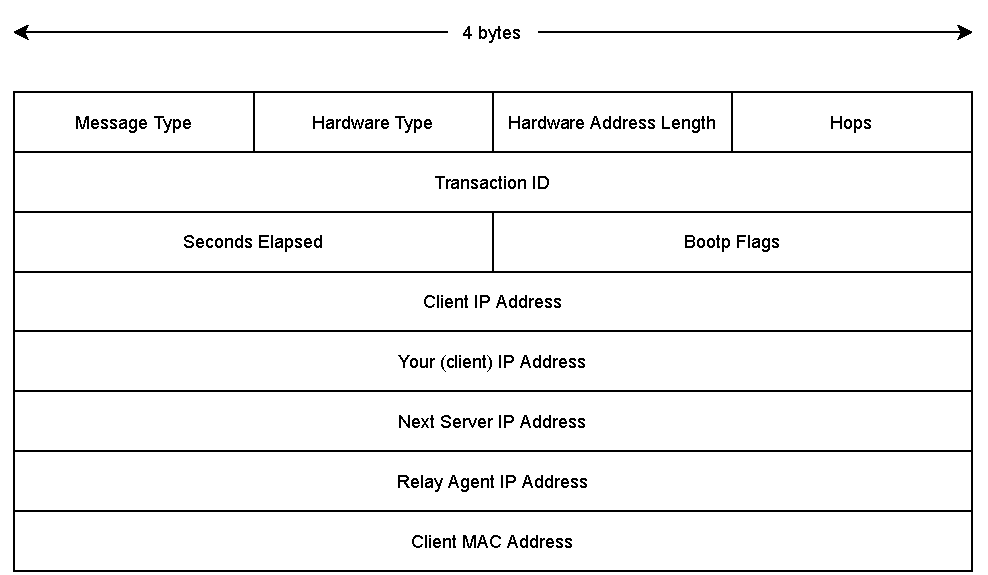
\includegraphics[width=\linewidth]{\imagesPath/2.7.pdf}
			\end{figure}

		\subsection*{2.8}
			Γίνεται κατανοητό από το πεδίο \verb|Magic Cookie|, το οποίο περιέχει τους αριθμούς 99, 130, 83 και 99 όταν πρόκειται για μήνυμα DHCP.

		\subsection*{2.9}
			Τα μηνύματα DHCP αυτά μεταφέρουν Boot Requests/Replies.

		\subsection*{2.10}
			Πριν τις επιλογές DHCP υπάρχουν επιπλέον τα:
			 
			\begin{itemize}
				\item Padding
				\item Server Host Name
				\item Boot File Name
				\item Magic Cookie
			\end{itemize}

		\subsection*{2.11}
			\begin{itemize}
				\item Όνομα: DHCP Message Type
				\item Κωδικός: 53
			\end{itemize}

		\subsection*{2.12}
			\begin{itemize}
				\item DHCP Release
					\begin{itemize}
						\item Length: 1
						\item DHCP: 7
					\end{itemize}
				\item DHCP Discover
					\begin{itemize}
						\item Length: 1 
						\item DHCP: 1
					\end{itemize}
				\item DHCP Offer
					\begin{itemize}
						\item Length: 1
						\item DHCP: 2
					\end{itemize}
				\item DHCP Request
					\begin{itemize}
						\item Length: 1
						\item DHCP: 3
					\end{itemize}
				\item DHCP ACK 
					\begin{itemize}
						\item Length: 1
						\item DHCP: 5
					\end{itemize}
			\end{itemize}

		\subsection*{2.13}
			Το πρώτο μήνυμα που έστειλε ο υπολογιστής μας ήταν DHCP Release, και σκοπό είχε να αποδεσμεύσει την IP Διεύθυνση που του είχε παραχωρήσει προσωρινά ο DHCP Server.

		\subsection*{2.14}
			Η διεύθυνση του αποστολέα ανήκει στον υπολογιστή μου και η διεύθυνση του παραλήπτη ανήκει στον DHCP Server/Default Gateway.

		\subsection*{2.15}
			\begin{itemize}
				\item Discover και Request:
					\begin{itemize}
						\item Src: \verb|3c:2c:30:e1:1c:55|
						\item Dst: \verb|ff:ff:ff:ff:ff:ff|
					\end{itemize}
			\end{itemize}

			\begin{itemize}
				\item Offer και ACK:
					\begin{itemize}
						\item Src: \verb|e0:0e:e4:59:40:50|
						\item Dst: \verb|3c:2c:30:e1:1c:55|
						
					\end{itemize}
			\end{itemize}
			
		\subsection*{2.16}
			\begin{itemize}
				\item Discover και Request:
				\begin{itemize}
					\item Src: \verb|0.0.0.0|
					\item Dst: \verb|255.255.255.255|
				\end{itemize}
			\end{itemize}
			
			\begin{itemize}
				\item Offer και ACK:
				\begin{itemize}
					\item Src: \verb|192.168.1.1|
					\item Dst: \verb|192.168.1.15|
					
				\end{itemize}
			\end{itemize}

		\subsection*{2.17}
			Η διεύθυνση παραλήπτη του DHCP Discover υποδηλώνει ότι έχουμε broadcast.

		\subsection*{2.18}
			Αυτό είναι λογικό, αφού ο υπολογιστής μας δεν έχει ακόμα διεύθυνση IPv4 στο τοπικό δίκτυο.

		\subsection*{2.19}
			Προτείνει την διεύθυνση 192.168.1.15, η οποία βρίσκεται στο πεδίο "Your (client) IP Address".

		\subsection*{2.20}
			Το προηγούμενο μήνυμα DHCP Offer στάλθηκε στην διεύθυνση \verb|192.168.1.15| ~/~  \verb|3c:2c:30:e1:1c:55|.

		\subsection*{2.21}
			Ναι, είναι σύμφωνες, αφού ο πελάτης έχει θέσει το Broadcast Flag ίσο με 0, και ο DHCP Server εκμπέμπει μόνο στην διεύθυνση IPv4 του υπολογιστή μας.

		\subsection*{2.22}
			Η διεύθυνση IPv4 του DHCP Server είναι 192.168.1.1 και βρίσκεται στο option "DHCP Server Identifier" (κωδικός 54).

		\subsection*{2.23}
			Η διεύθυνση IPv4 που ζητάει ο υπολογιστής μας είναι 192.168.1.15 και βρίσκεται στο option "Requested IP Address" (κωδικός 50).

		\subsection*{2.24}
			Το DHCP Request στέλνεται προς την MAC διεύθυνση \verb|ff:ff:ff:ff:ff:ff| και IPv4 διεύθυνση \verb|255.255.255.255|, όμως ο DHCP Server αναγνωρίζει ότι το μήνυμα απευθύνεται σε αυτόν από το option "DHCP Server Identifier".

		\subsection*{2.25}
			Τελικά στον υπολογιστή μας αποδίδεται η διεύθυνση 192.168.1.15 και αυτό φαίνεται από το πεδίο "Your (client) IP Address" του DHCP ACK.

		\subsection*{2.26}
			Ναι, συμπίπτει. 

		\subsection*{2.27}
			Η μάσκα υποδικτύου είναι \verb|255.255.255.0| και αυτό φαίνεται στο option "Subnet Mask".

		\subsection*{2.28}
			Η εκχώρηση της διεύθυνσης IPv4 διαρκεί 1 ημέρα και αυτό φαίνεται από το πεδίο "IP Address Lease Time".

		\subsection*{2.29}
			Ο κωδικός της επιλογής Parameter Request List είναι 55.

		\subsection*{2.30}
			\begin{itemize}
				\item 1 - Subnet Mask - Η τιμή της μάσκας υποδικτύου
				\item 26 - Interface MTU - Η MTU της δικτυακής διεπαφής
				\item 2 - Time Offset - Time Offset σε δευτερόλεπτα από το UTC.
			\end{itemize}

		\subsection*{2.31}
			Ο υπολογιστής μας ζητάει 13 παραμέτρους, ενώ ο εξυπηρετητής προσδιορίζει τις:
			
			\begin{itemize}
				\item 1 - Subnet Mask
				\item 3 - Router 
				\item 6 - Domain Name Server
				\item 15 - Domain Name
			\end{itemize} 

		\subsection*{2.32}
			Η σύνταξη του νέου φίλτρου απεικόνισης είναι \verb+dhcp || (arp && eth.src == 3c:2c:30:e1:1c:55)+.

		\subsection*{2.33}
			Όχι, δεν παρατηρώ.		

		\subsection*{2.34}
			N/A

		\subsection*{2.35}
			N/A

		\subsection*{2.36}
			N/A

		\subsection*{2.37}
			Παρήχθησαν DHCP Request και DHCP ACK.

		\subsection*{2.38}
			Όχι, τόσο τα πλαίσια Ethernet όσο και τα πακέτα IPv4 δεν διαφέρουν. 

		\subsection*{2.39}
			Η διεύθυνση που αιτείται ο υπολογιστής μας είναι η ίδια με πριν. Βρίσκεται στο option Requested IP Address.

		\subsection*{2.40}
			Η διεύθυνση της οποίας την ανανέωση εγκρίνει ο DHCP server ειαι ίδια με πριν, και βρίσκεται στο πεδίο "Your (client) IP Address".

		\subsection*{2.41}
			Είναι \verb|0x10b7b528|.

		\subsection*{2.42}
			Είναι \verb|0xa2b56775|.

		\subsection*{2.43}
			Είναι \verb|0x2e719d53|.

		\subsection*{2.44}
			Το Transaction ID έχει σκοπό να ομαδοποιήσει την κάθε ακολουθία μηνυμάτων μεταξύ πελάτη και εξυπηρετητή, και άρα να διαχωρίσει τις ακολουθίες μεταξύ τους. 
\end{document}